\chapter{Results}
\lhead{Results}
\rhead{Radu-George Rusu}
\label{Results}

The Airbus Ship Dataset Challenge \cite{AirbusDataSetChallenge} offers an automatic method of evaluation that, for every solution, computes the $F_2$ score. In order to avoid leader-board probing (competitors trying to over-fit the model on the test data), the test data set is split in two datasets. A public test dataset that contains $12\%$ of the original test images, and a private test dataset that contains the other, $88\%$ of the original test images.

To have a base model for comparison against the presented solutions, a No-Machine algorithm has been chosen. This algorithm evaluates every pixel as being a background pixel (no detection involved). The $F_2$ score for this algorithm is actually a percentage of how many images doesn't have ships in the image.

In the image recognition area is known that neural networks behave well, so, another model was chosen to have a top score value for comparison. This model is a combination between a residual network (ResNet34) which classifies the image in ship/no-ship images, and for images that have ships a U-Net, trained in the same fashion as the U-Net solution presented in this thesis, for the final classification phase. For the rest of the section we will refer to this solution as Hybrid.
\begin{table}[h]
	\centering
	\begin{tabular}{|c|c|c|}
		\hline
		Method & Private Test Dataset & Public Test Dataset \\ \hline
		No-Machine & 0.76566	& 0.52090  \\ \hline
		Region Proposal & 0.78052	& 0.58810 \\ \hline
		U-Net & 0.78424	& 0.61663  \\ \hline
		Hybrid & 0.79396 & 0.62259 \\ \hline
	\end{tabular}
	\captionof{table}{Results on the competition score}
	\label{resultOnComp}
\end{table}

The table \ref{resultOnComp} presents the results as scored by the Kaggle automatic evaluation. Both of the proposed solution have a better score than the No-Machine algorithm, which means that the two proposed solutions correctly identify images that have ships and the ones that does not. The results of the two proposed solutions are similar on both datasets, with small improvements when using the U-Net solution. This improvement is happening because of the granularity that the U-Net is using over the region proposal solution, which uses hard-coded dimensions and positions for the crops that can became region proposal for final prediction. It is worth mentioning that the $F_2$ score, computed as described in \ref{DatasetChapter}, penalizes false negatives over no prediction, which explains the small difference between No-Machine and the proposed solutions. As seen in \ref{resultOnComp}, the two solution have the tendency to classify small pockets of pixels as ships, which will drastically decrease the $F_2$ score for that respective image. Both of the proposed solutions behave worse than the Hybrid solution. The Region Proposal solution has the same weakness of using bulk windows for predictions while the Hybrid solution, as the U-Net proposal, has the advantage of granularity because of the end network used. In the case of U-Net Proposal, due to the pixel exclusion phase, it loses some information from the picture when the pixels are turned black, which leads to a weaker final prediction.

\begin{figure}
	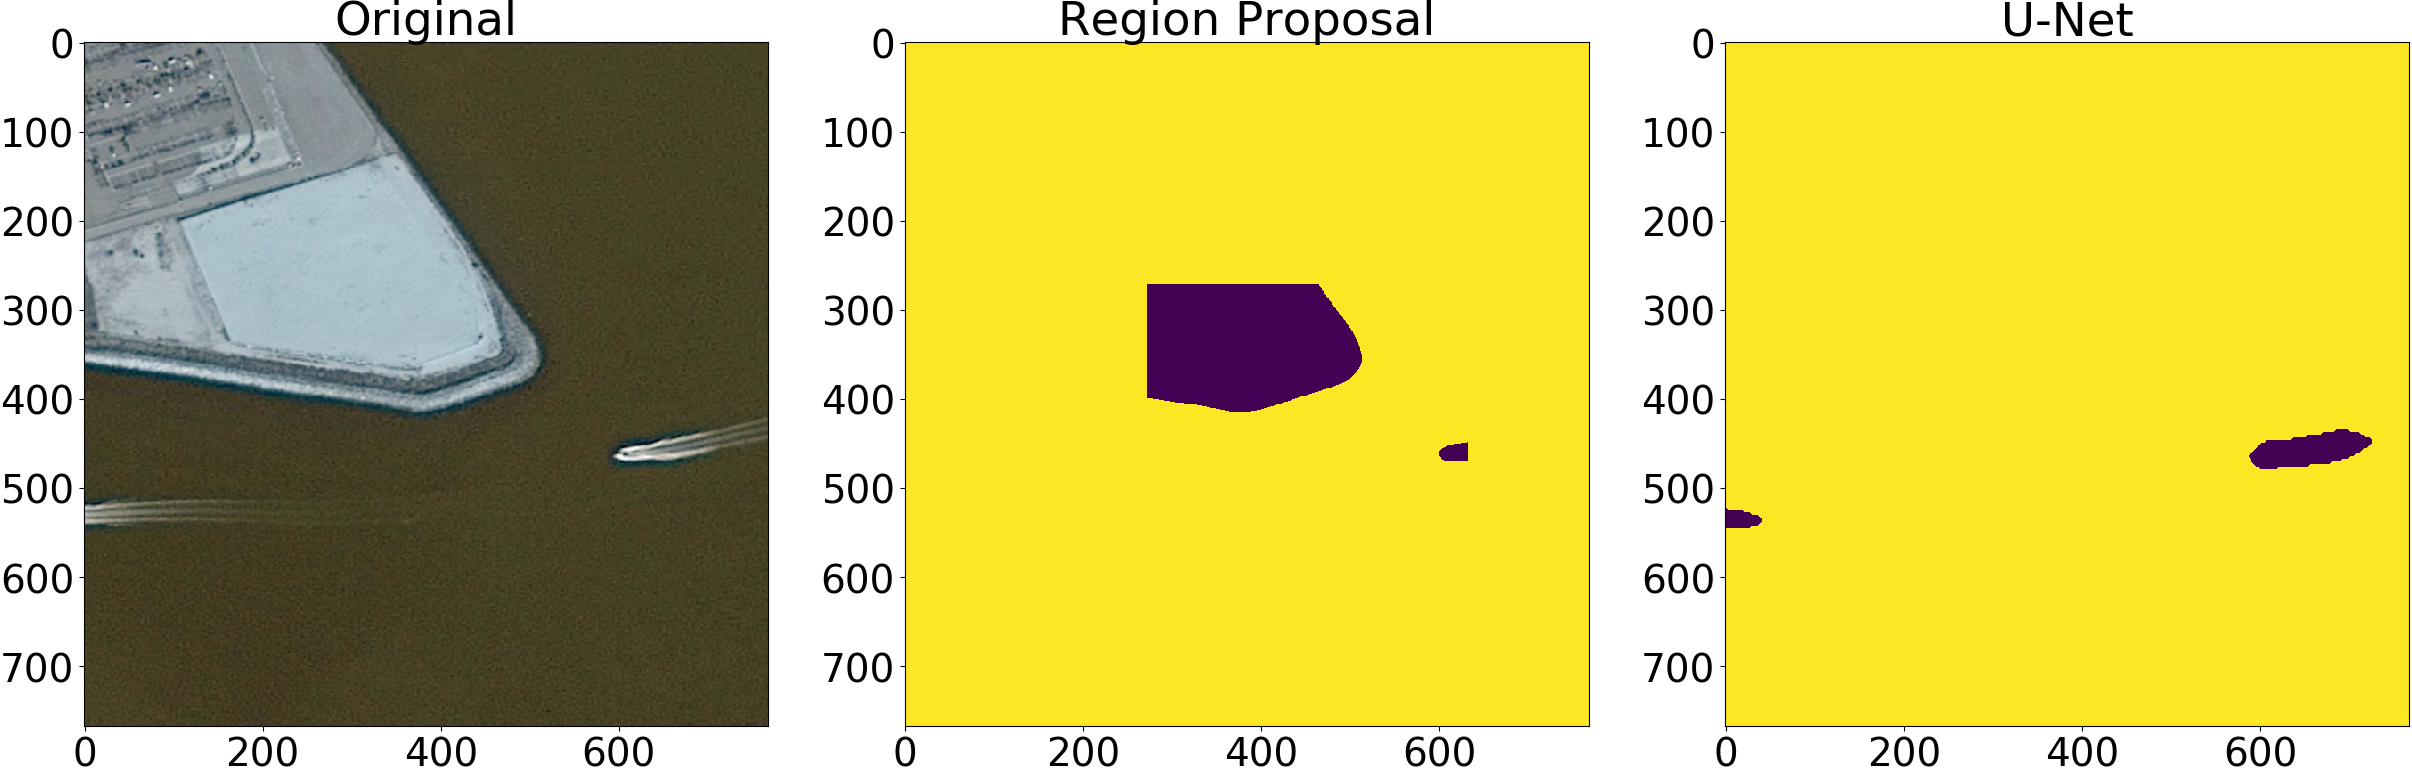
\includegraphics[width=\textwidth]{Pictures/016Comparison4.png}
	\caption{False Negative}
	\label{false_neg_size}
\end{figure}

Analyzing \ref{Final_Result}, the two algorithms, behaves in a similar fashion. The better behavior of the U-Net solution can be spotted since the false negatives produced by this, are smaller in area than the ones from the Region Proposal solution \ref{false_neg_size}. Again, the rigid character of the Region Proposal solution is seen in the \ref{false_neg_size}, where a big part of the port wasn't declassified because it was part of the same region with a ship inside, which the second Residual Network classified it as ship. Although from a visual perspective the U-Net architecture gives a better result, the $F_2$ score will be similar (not equal since the two predictions have different area of the ship mask).

\begin{figure}[H]
	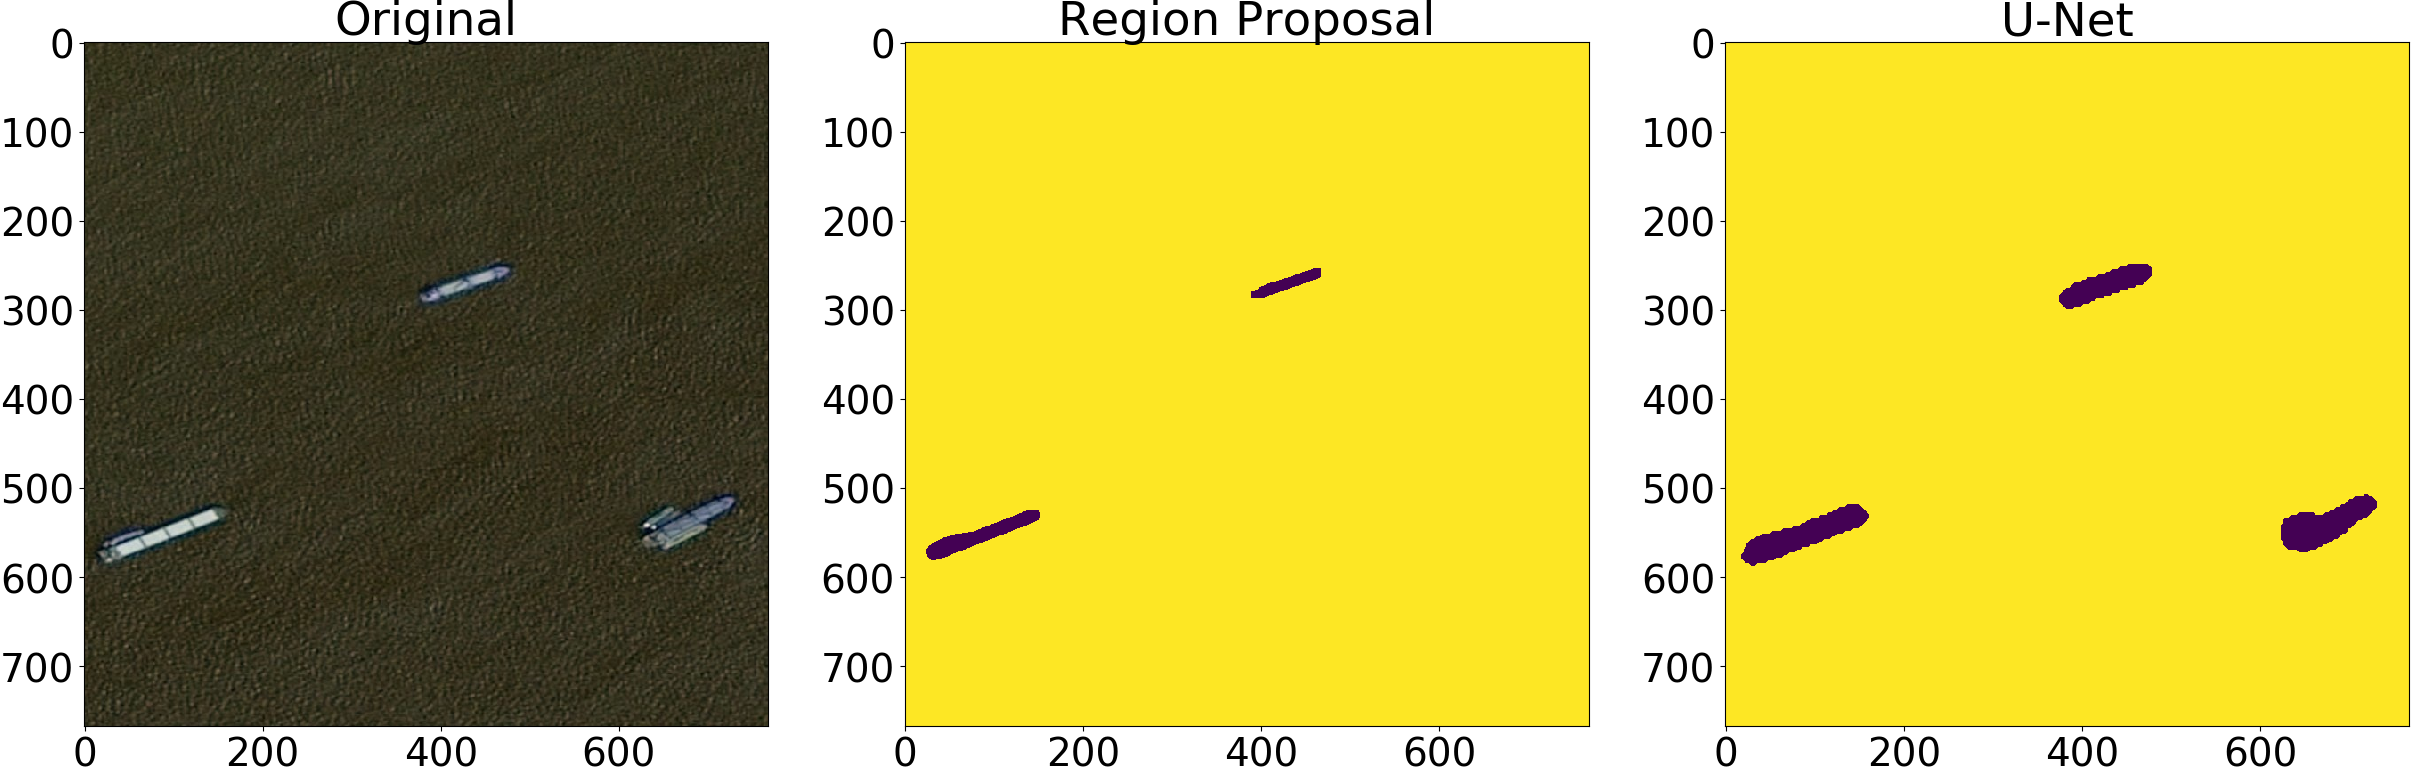
\includegraphics[width=\textwidth]{Pictures/016Comparison1.png}\\
	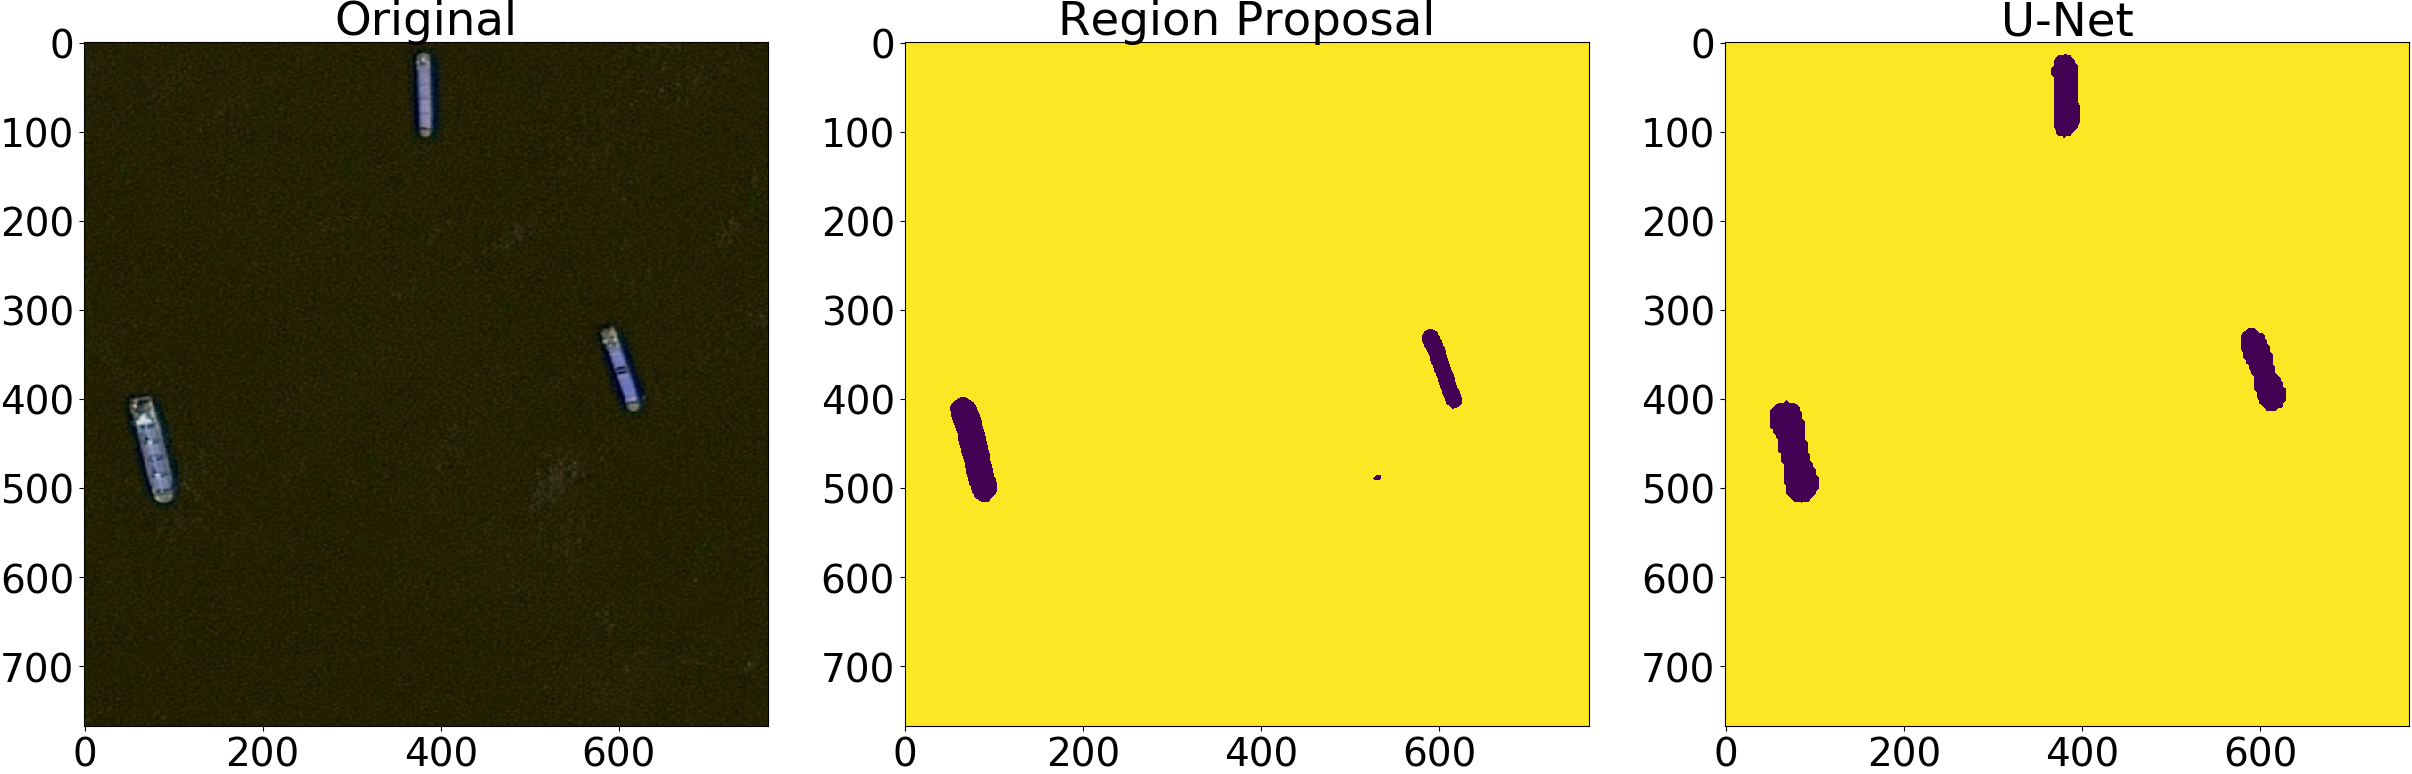
\includegraphics[width=\textwidth]{Pictures/016Comparison2.png}
	\caption{False Positive}
	\label{false_positive}
\end{figure}

Overall the two solutions are comparable in terms of $F_2$ score, but on a visual analysis of the results, the U-Net architecture produces less false positives \ref{false_positive} and false negatives. The figure \ref{Final_Result} presents a few more uses cases that confirms the above conclusions.

In the figure \ref{Final_Result_Port}, it is shown that pictures with ports are still a challenge for both solutions. The weak flexibility of the region proposal determined by using bulk windows, can be spotted when a ship is presented in the same window with a piece/or multiple pieces of the port, which in turn also leads to a lot of false negatives. The U-Net solution also struggles to differentiate the port from the ships, the results detection having a lot of pockets that will be evaluate as false negatives and in turn a smaller $F_2$ score.

\begin{figure}
	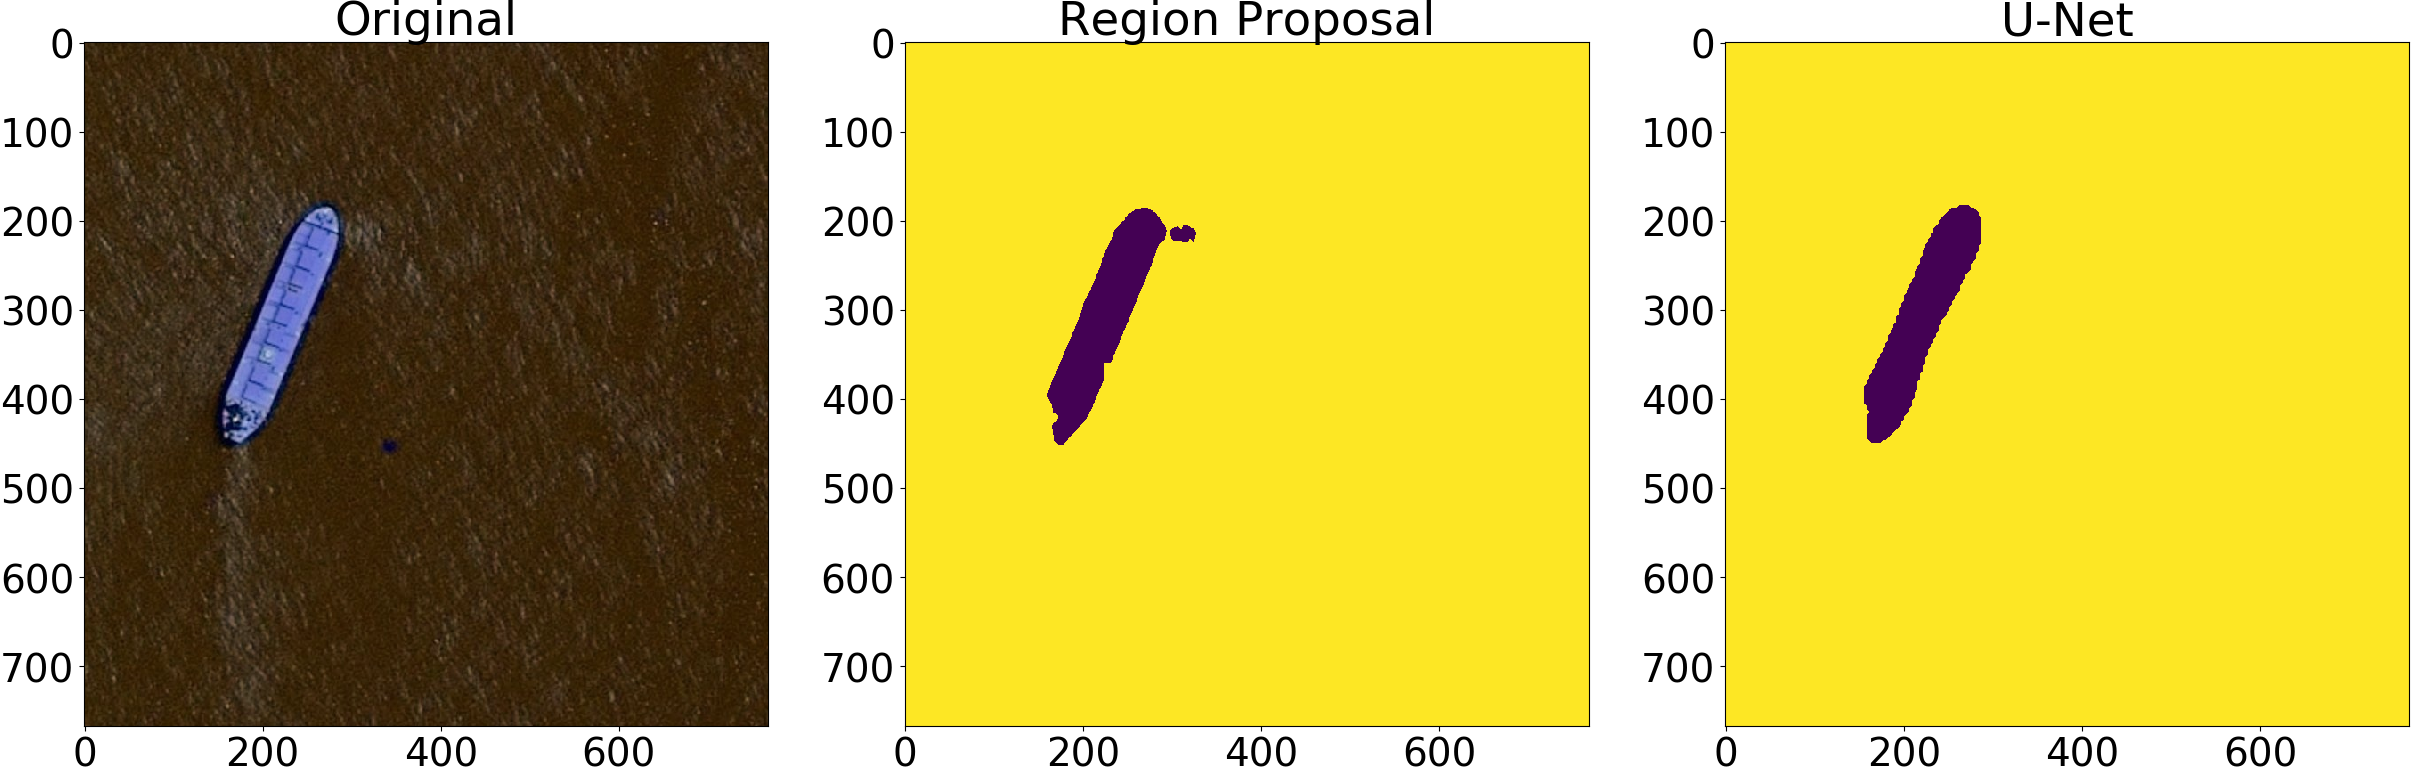
\includegraphics[width=0.9\textwidth]{Pictures/016Comparison3.png}
	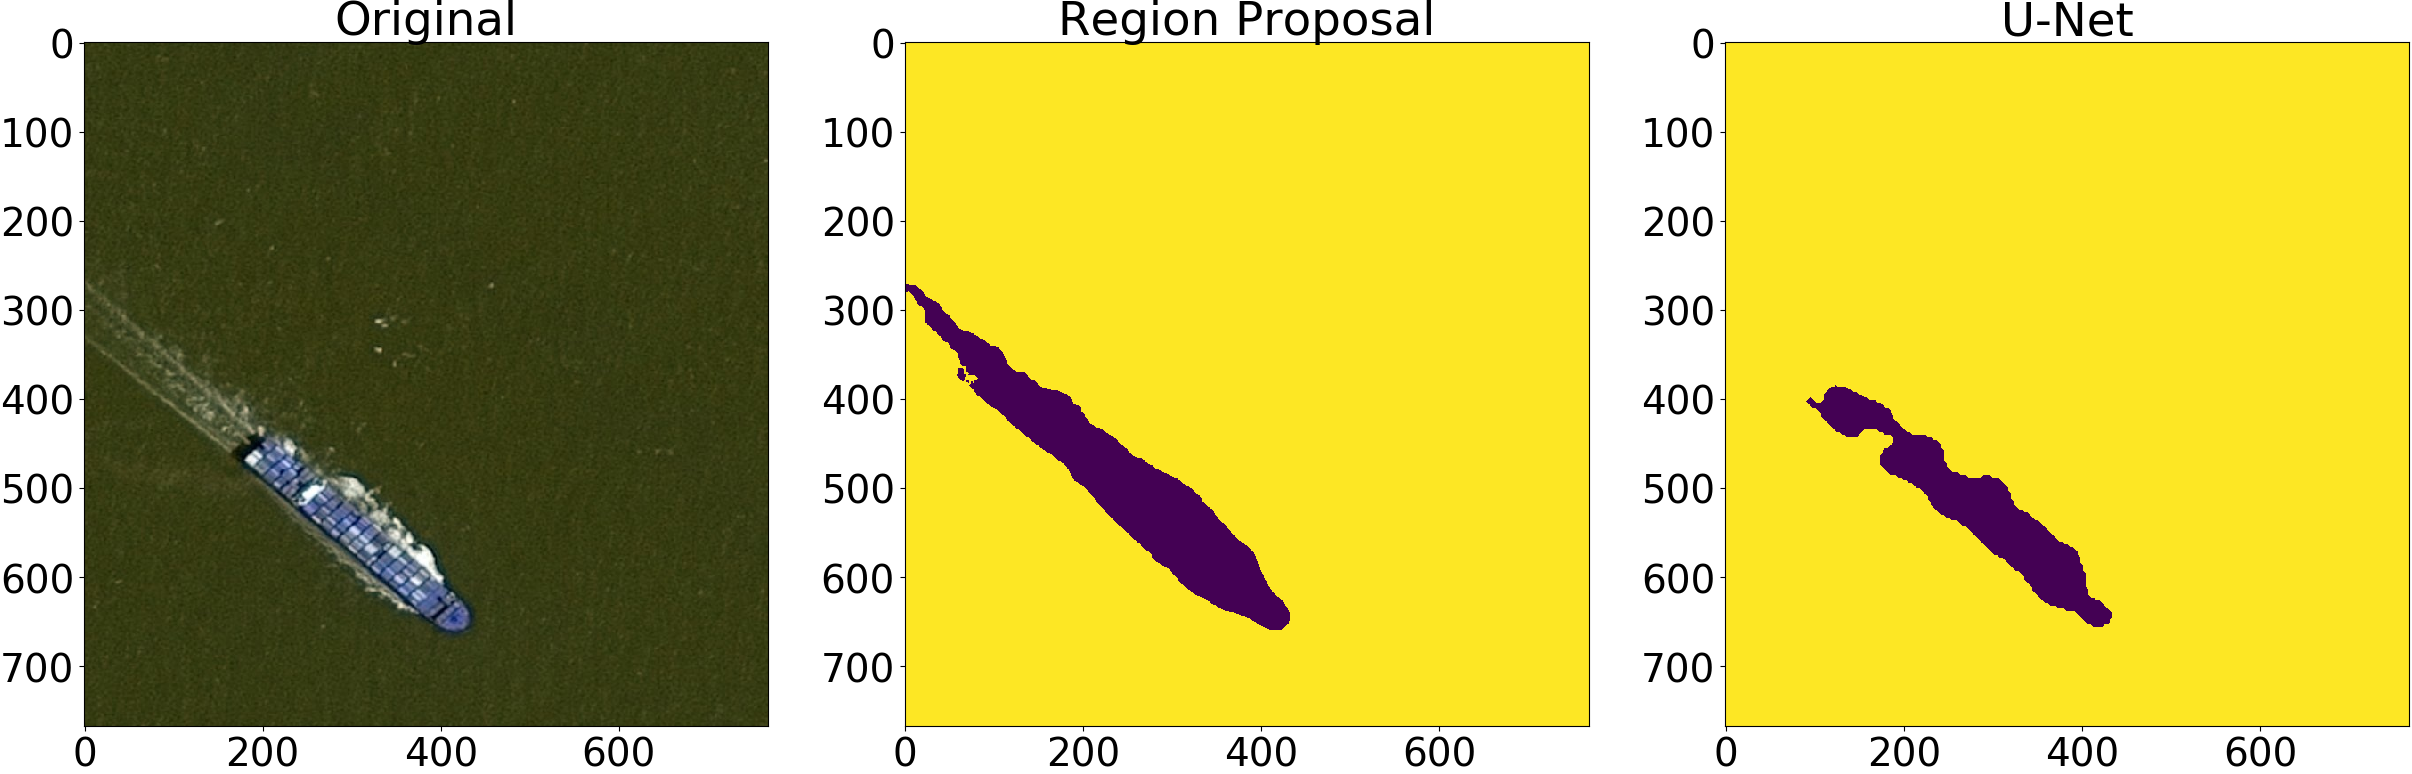
\includegraphics[width=0.9\textwidth]{Pictures/016Comparison5.png}
	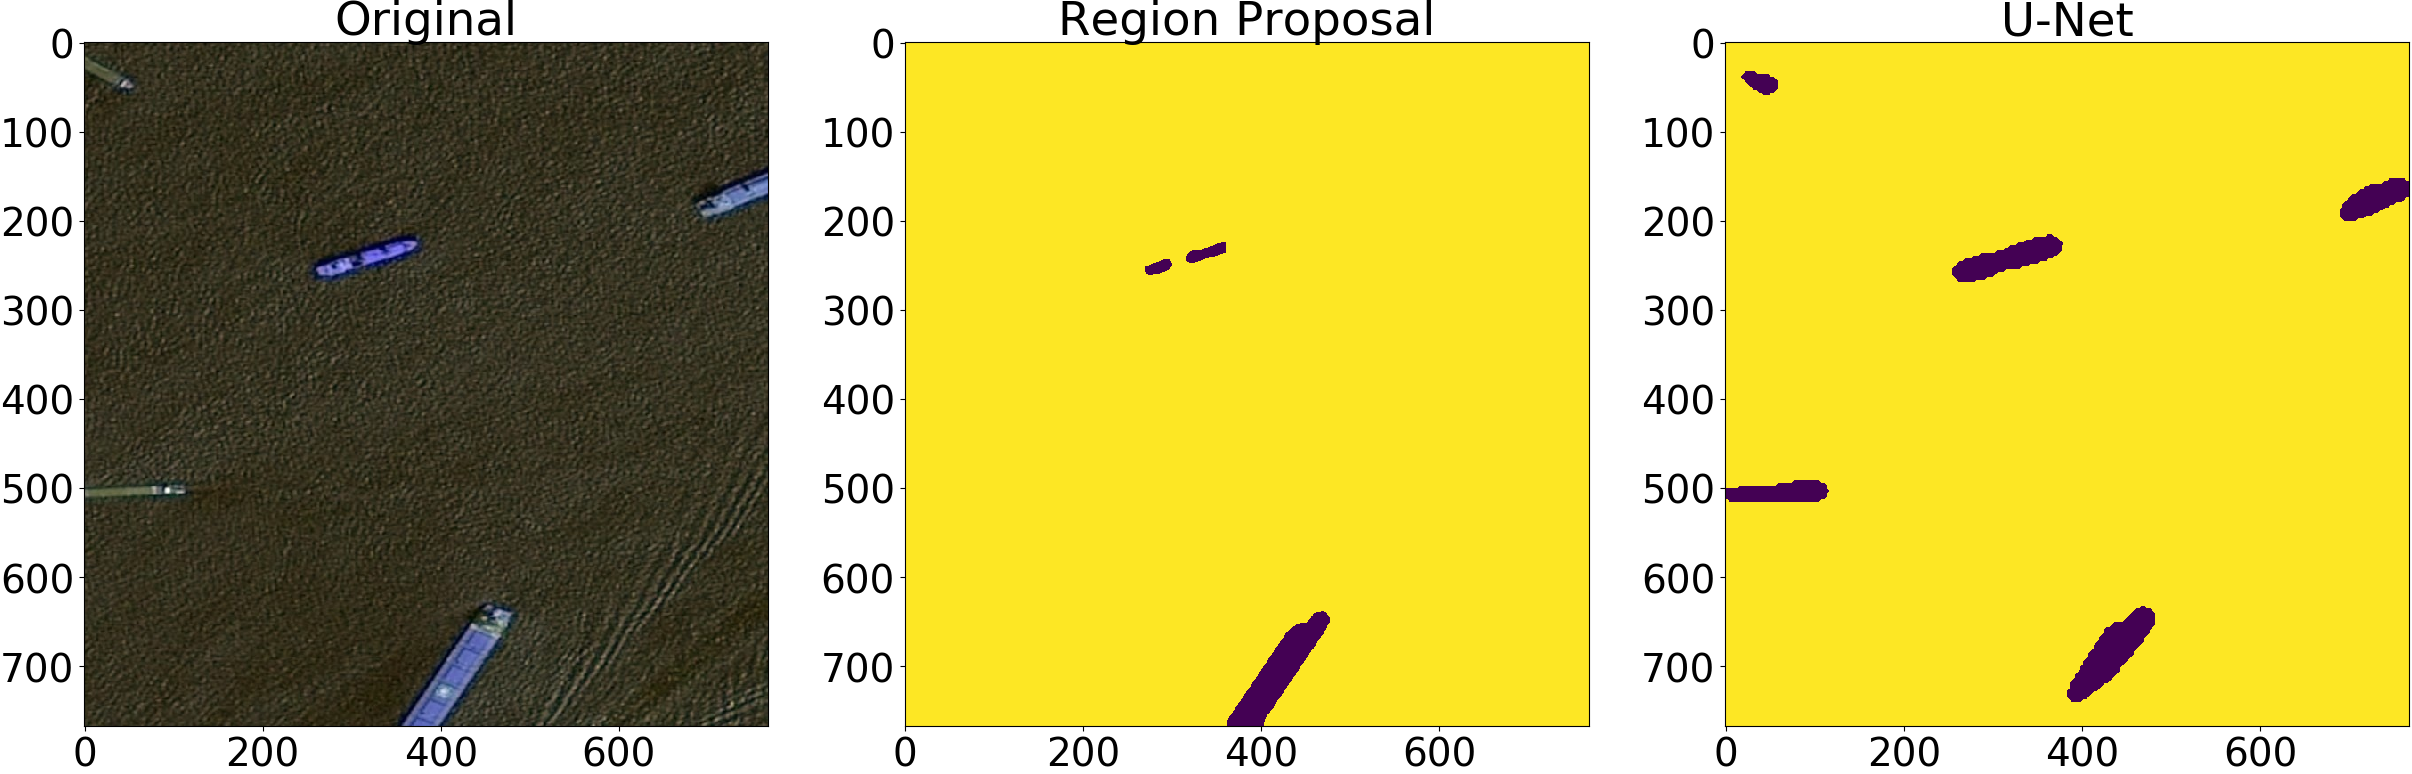
\includegraphics[width=0.9\textwidth]{Pictures/016Comparison6.png}
	\caption{Final Result comparison}
	\label{Final_Result}
\end{figure}

\begin{figure}
	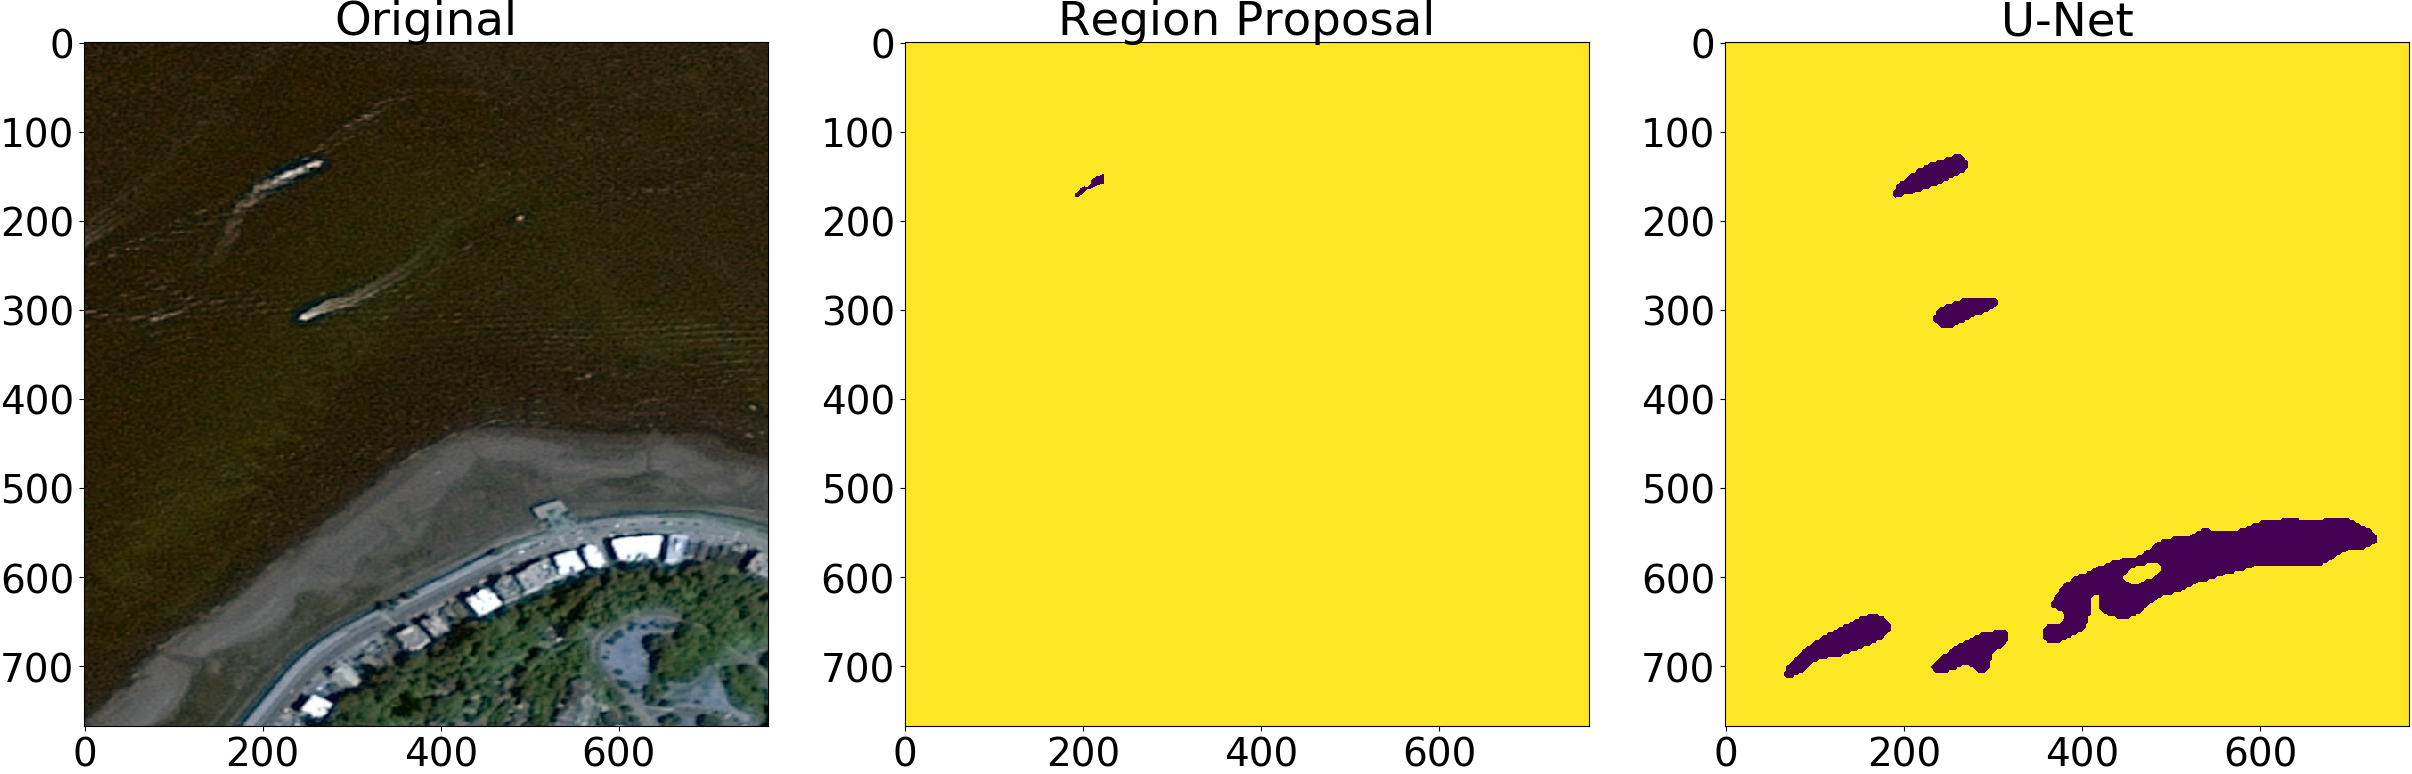
\includegraphics[width=0.9\textwidth]{Pictures/016Comparison7.png}
	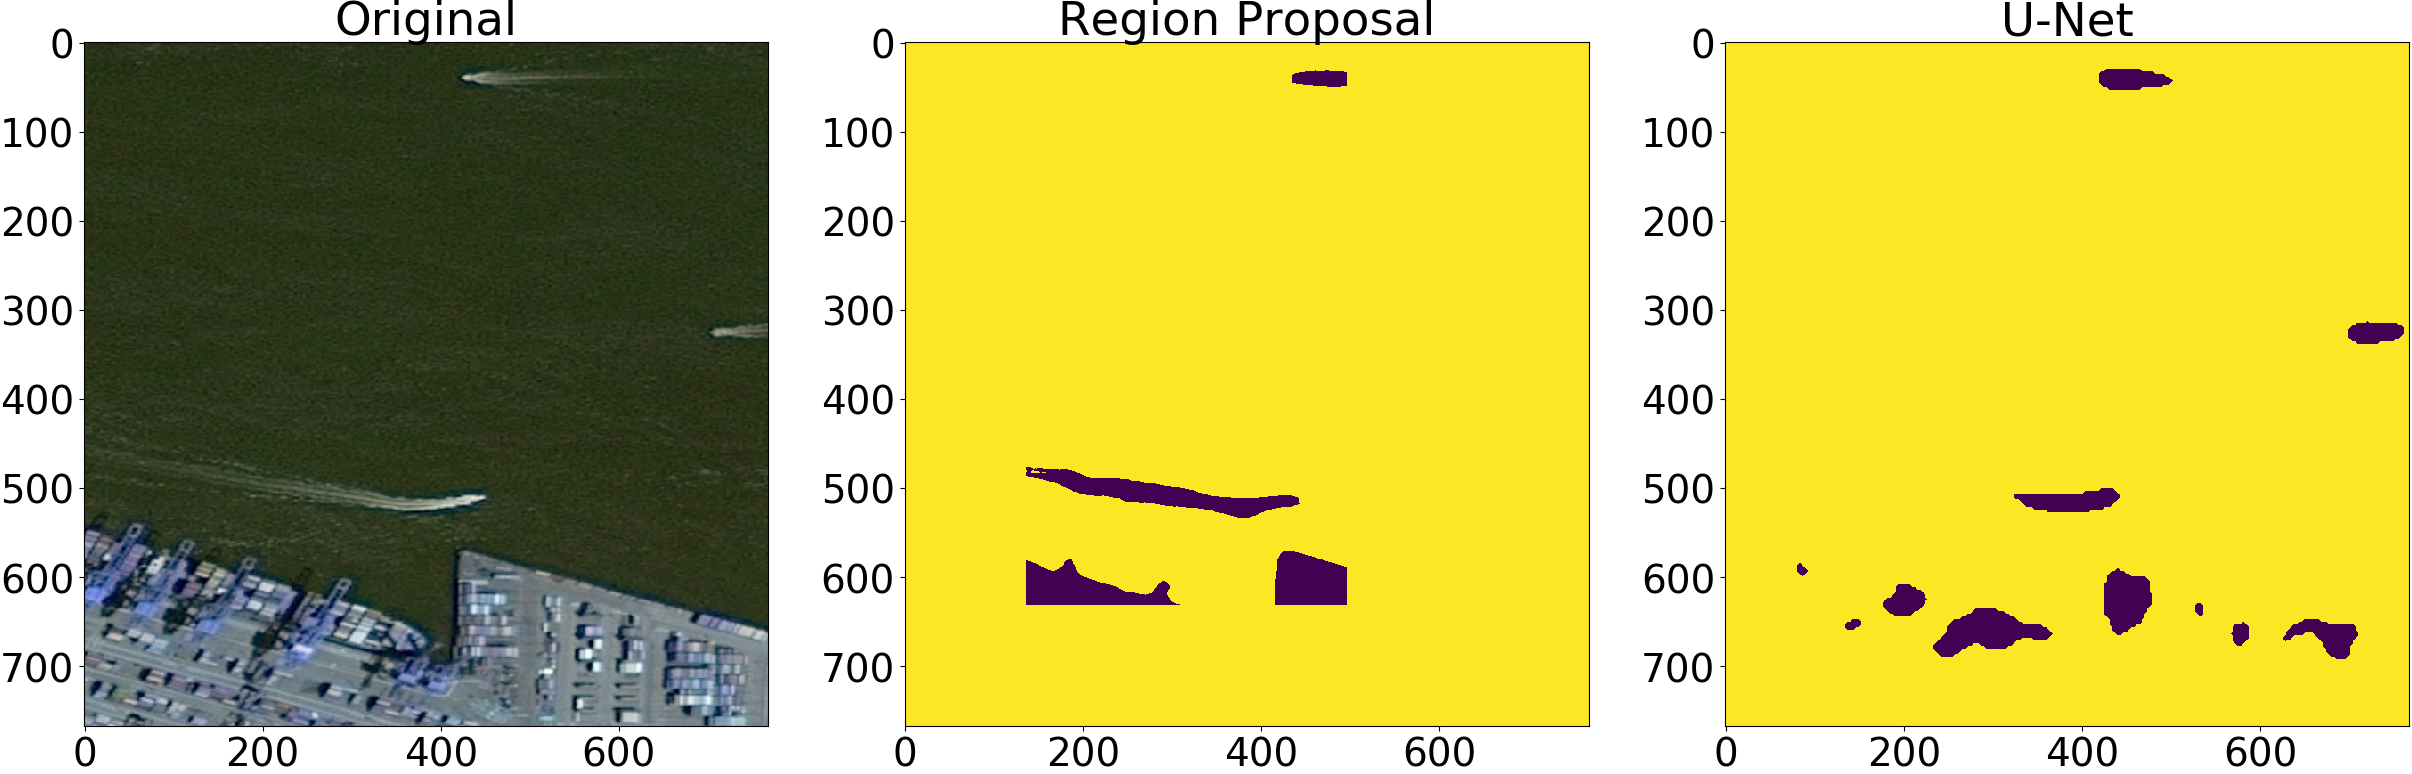
\includegraphics[width=0.9\textwidth]{Pictures/016Comparison8.png}
	\caption{Final Result Port Comparison}
	\label{Final_Result_Port}
\end{figure}